\documentclass[border=8pt,tikz]{standalone}
\usepackage{tikz}
% Shared TikZ style for Chapter 5 diagrams.
% Inputted by every standalone diagram file.

\usetikzlibrary{
  arrows.meta,
  positioning,
  shapes.geometric,
  shapes.symbols,
  shapes.multipart,
  shapes.misc,
  fit,
  calc,
  backgrounds,
  decorations.pathmorphing,
  decorations.pathreplacing,
  patterns,
  shadows.blur,
}

% ─── Colour palette ──────────────────────────────────────────────
\definecolor{strixBlue}{HTML}{3B7DD8}     % data sources / inputs
\definecolor{strixGreen}{HTML}{22A699}    % processing / workers
\definecolor{strixOrange}{HTML}{E08036}   % storage
\definecolor{strixRed}{HTML}{E04B4B}      % attacker / external threat
\definecolor{strixPurple}{HTML}{6B5DD3}   % frontend / UI
\definecolor{strixGold}{HTML}{F2BE22}     % models / ML
\definecolor{strixGrey}{HTML}{6E7681}     % neutral / labels
\definecolor{strixDark}{HTML}{1F2933}     % titles / borders

% ─── Common node styles ──────────────────────────────────────────
\tikzset{
  >={Latex[width=2mm,length=2.5mm]},
  font=\sffamily\small,
  every node/.style={align=center},
  comp/.style={
    rectangle, rounded corners=2pt, draw=#1, fill=#1!10, very thick,
    text=strixDark, minimum width=22mm, minimum height=8mm,
    inner sep=4pt,
  },
  comp/.default=strixGreen,
  store/.style={
    cylinder, shape border rotate=90, aspect=0.3, draw=strixOrange,
    fill=strixOrange!12, very thick, text=strixDark,
    minimum width=18mm, minimum height=10mm, inner sep=2pt,
  },
  stream/.style={
    rectangle, rounded corners=2pt, draw=strixOrange,
    fill=strixOrange!8, dashed, thick, text=strixDark,
    minimum width=22mm, minimum height=7mm, inner sep=3pt,
    font=\ttfamily\scriptsize,
  },
  source/.style={comp=strixBlue},
  worker/.style={comp=strixGreen},
  model/.style={comp=strixGold},
  ui/.style={comp=strixPurple},
  ext/.style={comp=strixRed},
  title/.style={font=\sffamily\bfseries, text=strixDark},
  edge/.style={->, thick, draw=strixGrey, font=\sffamily\scriptsize\itshape},
  edgeStrong/.style={->, very thick, draw=strixDark, font=\sffamily\scriptsize\bfseries},
  group/.style={
    rectangle, rounded corners=4pt, draw=strixGrey, dashed, thick,
    inner sep=6pt, fill=strixGrey!4,
  },
  badge/.style={
    rectangle, rounded corners=1pt, fill=#1, text=white,
    font=\sffamily\scriptsize\bfseries, inner sep=2pt,
  },
  badge/.default=strixDark,
  port/.style={
    rectangle, rounded corners=1pt, draw=strixDark, fill=strixGrey!8,
    font=\ttfamily\scriptsize, minimum width=14mm, inner sep=2pt,
  },
}


\begin{document}
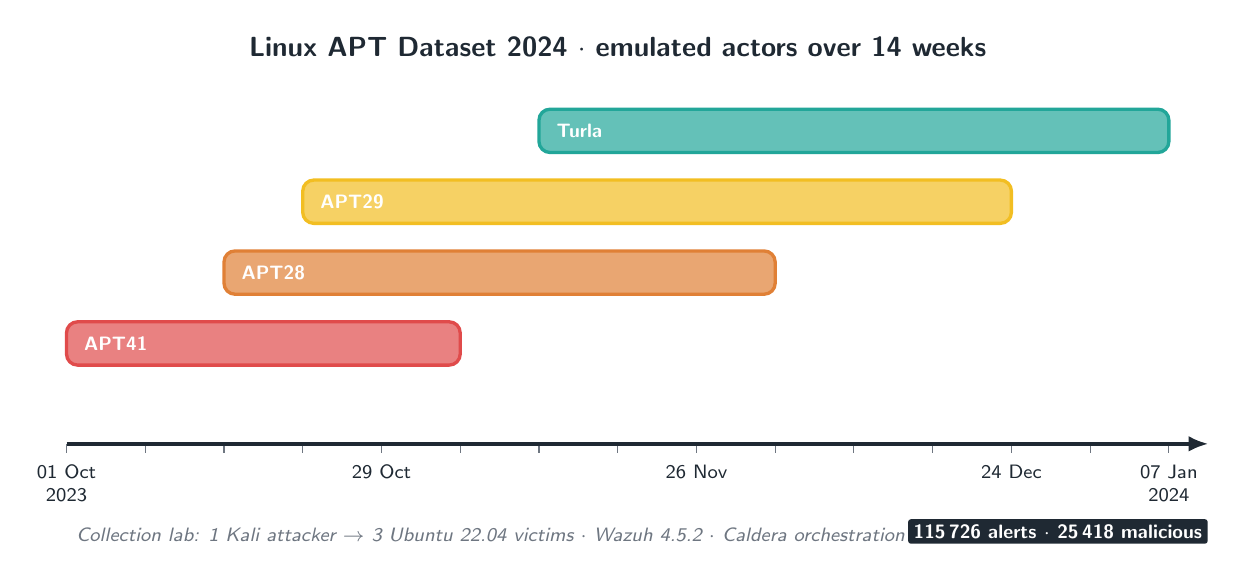
\begin{tikzpicture}[x=1cm, y=1cm]

% ─── Time axis: Oct 2023 → Jan 2024 (14 weeks) ────────────────────
\def\W{1.0}                          % 1cm per week
\def\WEEKS{14}
\def\AXISY{0}

% Ticks for week boundaries (every 2 weeks labelled)
\foreach \w in {0,...,14} {
  \draw[draw=strixGrey] (\w*\W,\AXISY) -- (\w*\W,\AXISY-0.12);
}
\foreach \w/\lbl in {0/{01 Oct\\2023}, 4/{29 Oct}, 8/{26 Nov}, 12/{24 Dec}, 14/{07 Jan\\2024}} {
  \node[font=\sffamily\scriptsize, text=strixDark, anchor=north]
    at (\w*\W, \AXISY-0.15) {\lbl};
}
\draw[very thick, draw=strixDark, ->] (0,\AXISY) -- (\WEEKS*\W+0.5,\AXISY);

% ─── Ribbons: one per APT actor, stacked above the axis ───────────
% Format: name / colour / start week / end week / row (0=closest to axis)
\foreach \name/\col/\s/\e/\r in {
  APT41/strixRed/0/5/0,
  APT28/strixOrange/2/9/1,
  APT29/strixGold/3/12/2,
  Turla/strixGreen/6/14/3%
} {
  \pgfmathsetmacro{\Y}{1.0 + \r*0.9}
  \fill[\col!70, rounded corners=4pt]
    (\s*\W,\Y) rectangle (\e*\W, \Y+0.55);
  \draw[draw=\col, very thick, rounded corners=4pt]
    (\s*\W,\Y) rectangle (\e*\W, \Y+0.55);
  \node[font=\sffamily\bfseries\scriptsize, text=white, anchor=west]
    at (\s*\W+0.1, \Y+0.27) {\name};
}

% ─── Annotation: total volume + collection note ──────────────────
\node[font=\sffamily\scriptsize\itshape, text=strixGrey, anchor=north west]
  at (0, \AXISY-0.95)
  {Collection lab: 1 Kali attacker $\to$ 3 Ubuntu 22.04 victims \(\cdot\) Wazuh 4.5.2 \(\cdot\) Caldera orchestration};
\node[badge=strixDark, anchor=north east]
  at (\WEEKS*\W+0.5,\AXISY-0.95) {115\,726 alerts \(\cdot\) 25\,418 malicious};

\node[font=\sffamily\bfseries, anchor=south, text=strixDark]
  at (\WEEKS*\W*0.5, 4.8) {Linux APT Dataset 2024 \(\cdot\) emulated actors over 14 weeks};

\end{tikzpicture}
\end{document}
